\documentclass{article}

\usepackage[vmarginratio=1:1,a4paper,body={6.5in, 9.5in}]{geometry}

\usepackage[T2A]{fontenc}
\usepackage[utf8]{inputenc}
\usepackage[russian]{babel}

\usepackage{wrapfig}

\usepackage{amsmath}
\DeclareMathOperator*{\argmin}{arg\,min}

\usepackage{amssymb}
\usepackage{amsfonts}
\usepackage{amsthm}
\newtheorem{theorem}{Theorem}
\newtheorem{definition}{Definition}

\usepackage{hyperref}
\usepackage{graphicx}
\graphicspath{{./img/}}


\begin{document}
\section{Is probability theory well-founded or do you believe in the theory of evolution?}

I’ll start with the least squares methods through the maximum likelihood estimation;
this requires some (at least superficial) knowledge of probability theory. 


\begin{wrapfigure}{r}{.2\linewidth}

\includegraphics[width=\linewidth]{stop-following-me}
\end{wrapfigure}
I was once asked if I believed in evolutionary theory. 
Take a short break, think about how you would answer.
Being puzzled by the question, I have answered that I find it plausible. 
Scientific theory has little to do with faith.
In short, a theory only builds a model of the world, and there is no need to believe in it.
Moreover, the Popperian criterion\cite{} requires a scientific theory be able to be falsifiable. 
A solid theory must possess, first of all, the power of prediction.
For example, if you genetically modify crops in such a way that they produce pesticides themselves, 
it is only logical that pesticide-resistant insects would appear. 
However, it is much less obvious that this process can be slowed down by growing regular plants side by side with genetically modified plants. 
Based on evolutionary theory, the corresponding modelling has made this prediction\cite{}, and it seems to have been validated\cite{}.

\paragraph*{Wait, what is the conection?}

As I mentioned earlier, the idea is to approach the least squares through the principle of maximum likelihood. 
Let us illustrate by example. 
Suppose we are interested in penguins body height, but we are only able to measure a few of these magestic birds.
It is reasonable to introduce the body height distribution model into the task; most often it is supposed to be normal.
A normal distribution is characterized by two parameters: the average value and the standard deviation.
For each fixed value of parameters, we can calculate the probability that the measurements we made would be generated.
Then, by varying the parameters, we will find those that maximize the probability.



$$P(a) = .4  \qquad  P(a\wedge b) = 0 \qquad P(b) = .3 \qquad P(a\vee b) = .8$$
	
\begin{tabular}{cccccc}
	\multicolumn{2}{c}{Bets of the Agent 2}  &  \multicolumn{4}{c}{Result for the Agent 1} \\
	\hline
	{\tiny Event} & {\tiny Bet amount} & {\tiny $a\wedge b$} & {\tiny $a\wedge \neg b$} &  {\tiny $\neg a\wedge b$} &  {\tiny $\neg a\wedge\neg b$} \\
	\hline
	$a$             & 4-6 & -6 & -6 &  4 &  4 \\
	$b$             & 3-7 & -7 &  3 & -7 &  3 \\
	$\neg(a\vee b)$ & 2-8 &  2 &  2 &  2 & -8 \\
	\hline
	&     &-11 & -1 & -1 & -1
\end{tabular}
	
\begin{itemize}
	\item $0\leq P(a)\leq 1$
	\item $P(true)=1$, $P(false) = 0$
	\item $P(a\vee b) = P(a) + P(b) - P(a\wedge b)$
\end{itemize}

In text form, they look like this:
\begin{enumerate}
\item All probabilities range from 0 to 1.
\item Certainly true statements have probability of 1 and certainly false probability of 0.
\item The third axiom is the very intuitive disjunction axiom.
All cases where the statement $a$ is true, together with those where $b$ is true,
cover all those cases where the statement $a\vee b$ is true; however the intersection $a\wedge b$ is counted twice in the sum, therefore it is necessary to subtract $P(a\wedge b)$.
\end{enumerate}

In 1931, de Finetti proved a very strong proposition:

\vspace{4mm}

\textit{If a bookmaker is guided by beliefs which break the axioms of the theory of probability,
then there exists such a combination of bets of the player which guarantees the loss for the bookmaker (a prize for the player) at each bet.
}

\vspace{4mm}

Probability axioms can be considered as the limiting set of probabilistic beliefs that some agent can adhere to.
Note that if a bookmaker respects Kolmogorov's axioms, it does not imply that he will win (leaving aside the fees),
however, if he does not respect the axioms, he is guaranteed to lose.
Other arguments have been put forward in favour of the probability theory;
but it is the practical success of probability-based reasoning systems that has proved to be very attractive.


\section{Maximum likelihood through examples}
\subsection{First example: coin toss}
Let us consider a simple example of coin flipping, also known as the Bernoulli's scheme. 
We conduct $n$ experiments, two events can happen in each one (``success'' or ``failure''): 
one happens with probability $p$, the other one with probability $1-p$. 
Our goal is to find the probability of getting exactly $k$ successes in these $n$ experiments. 
This probability is given by the Bernoulli's formula:
$$
P(k;n,p) = C_n^k p^k (1-p)^{n-k}
$$

Let us take an ordinary coin ($p=1/2$), flip it ten times ($n=10$), and count how many times we get the tails:
$$P(k) = C_{10}^k \frac{1}{2^k}\left(1-\frac{1}{2}\right)^{n-k} = \frac{C_{10}^k}{2^n}$$
Figure~\ref{fig:binomial}, left shows what a probability density graph looks like.

\begin{figure}[htb!]
\centering
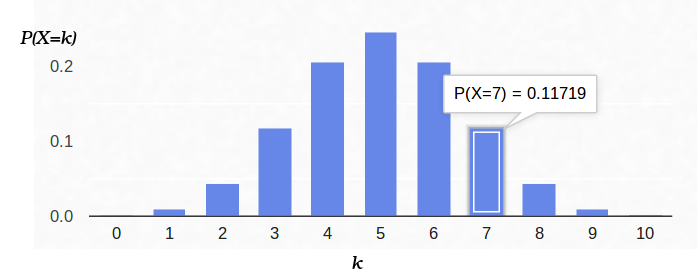
\includegraphics[width=.48\columnwidth]{binomial-05}
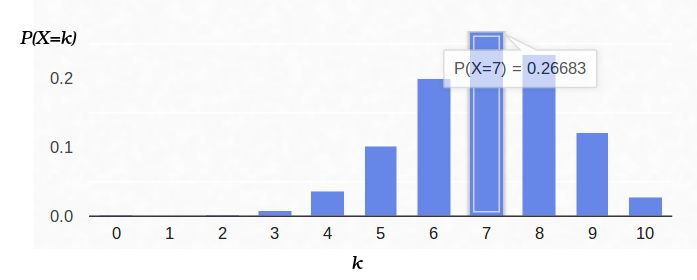
\includegraphics[width=.48\columnwidth]{binomial-07}
\caption{\textbf{Left:} probability density graph for the Bernoulli's scheme with $p=1/2$. \textbf{Right:} probability density graph for the Bernoulli's scheme with $p=7/10$.}
\label{fig:binomial}
\end{figure}

Thus, if we have fixed the probability of ``success'' ($1/2$) and also fixed the number of experiments (10), 
then the possible number of ``successes'' can be any integer between 0 and 10, but these outcomes are not equiprobable. 
It is clear that five ``successes'' are much more likely to happen than none. For example, the probability encountering seven tails is about 12\%.

Now let us look at the same problem from a different angle. 
Suppose we have a real coin, but we do not know its distribution of a priori probability of ``success''/``failure''. 
However, we can toss it ten times and count the number of ``successes''. 
For example, we have counted seven tails.
Would it help us to evaluate $p$?

We can try to fix $n=10$ and $k=7$ in the Bernoulli's formula, leaving $p$ as a free parameter:
$$\mathcal{L}(p) = C_{10}^7 p^7 (1-p)^3$$

Then the Bernoulli's formula can be interpreted as the plausibility of the parameter being evaluated (in this case $p$).
I have even changed the function notation, now it is denoted as $\mathcal L$ (likelihood).
That is being said, the likelihood is the probability to generate the observation data (7 tails out of 10 experiments) for the given value of the parameter(s).
For example, the likelihood of a balanced coin ($p=1/2$) with seven tails out of ten tosses is approximately 12\%. 
Figure~\ref{fig:likelihood} plots the likelihood function for the observation data with 7 tails out of 10 experiments.

\begin{figure}[htb!]
\centering
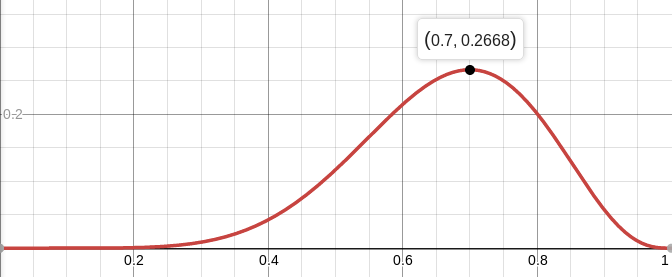
\includegraphics[width=.5\columnwidth]{likehood-07}
\caption{The plot of the likelihood function $\mathcal{L}(p)$ for the observation data with 7 tails out of 10 experiments.}
\label{fig:likelihood}
\end{figure}

So, we are looking for the parameter value that maximizes the likelihood of producing the observations we have.
In our particular case, we have a function of one variable, and we are looking for its maximum.
In order to make things easier, I will not search for the maximum of $\mathcal L$, but for the maximum of $\log \mathcal L$.
The logarithm is a strictly monotonous function, so maximizing both is equivalent.
The logarithm has a nice property of breaking down products into sums that are much more convenient to differentiate.
So, we are looking for the maximum of this function:
$$\log \mathcal{L}(p) = \log C_{10}^7 + 7 \log p + 3\log (1-p)$$

That's why we equate it's derivative to zero:
$$\frac{d \log \mathcal{L}}{dp} = 0$$

The derivative of $\log x = \frac{1}{x}$, therefore:
$$\frac{d \log \mathcal{L}}{dp} = \frac{7}{p} - \frac{3}{1-p} = 0$$

That is, the maximum likelihood (about 27\%) is reached at the point $p=7/10$.
Just in case, let us check the second derivative:
$$\frac{d^2 \log \mathcal{L}}{dp^2} = -\frac{7}{p^2} - \frac{3}{(1-p)^2}$$

In the point $p=7/10$ it is negative, therefore this point is indeed a maximum of the function $\mathcal{L}$:
$$\frac{d^2 \log \mathcal{L}}{dp^2}(0.7)  \approx -48 < 0$$

Figure~\ref{fig:binomial} shows the probability density graph for the Bernoulli's scheme with $p=7/10$.


\subsection{Second example: analog-to-digital converter (ADC)}

Let us imagine that we have a constant physical quantity that we want to measure; for example, it can be a length to measure with a ruler or a voltage with a voltmeter.
In the real world, any measurement gives \textit{an approximation} of this value, but not the value itself.
The methods I am describing here were developed by Gauss at the end of the 18th century, when he measured the orbits of celestial bodies
\footnote{Note that Legendre has published an equivalent method in 1805, 
whereas Gauss' first publication is dated by 1809. Gauss has always claimed that he had been using the method since 1795,
and this is a very famous priority dispute~\cite{https://projecteuclid.org/download/pdf_1/euclid.aos/1176345451} in the history of statistics.
There are, however, numerous evidence to support the thesis that Gauss possessed the method before Legendre, but he was late in his communication.}.
~\cite{Theoria Motus Corporum Coelestium}

For example, if we measure the battery voltage $N$ times, we get $N$ different measurements. Which of them should we take? All of them! 
So, let us say that we have $N$ measurements $U_j$:
$$
\{U_j\}_{j=1}^{N}
$$

Let us suppose that each measurement $U_j$ is equal to the real value plus the Gaussian noise. 
The noise is characterized by two parameters --- the center of the Gaussian bell and its ``width''. 
In this case, the probability density can be expressed as follows:
$$
p(U_j) = \frac{1}{\sqrt{2\pi}\sigma} \exp\left(-\frac{(U_j-U)^2}{2\sigma^2}\right)
$$

That is, having $N$ measurements $U_j$, our goal is to find the parameters $U$ and $\sigma$ that maximize the likelihood.
The likelihood (I have already applied the logarithm) can be written as follows:
\begin{align*}
\log \mathcal{L}(U,\sigma) & = \log \left(\prod\limits_{j=1}^N  \frac{1}{\sqrt{2\pi}\sigma} \exp\left(-\frac{(U_j-U)^2}{2\sigma^2}\right)\right) =\\
& = \sum\limits_{j=1}^N \log \left(\frac{1}{\sqrt{2\pi}\sigma} \exp\left(-\frac{(U_j-U)^2}{2\sigma^2}\right)\right) = \\
& = \sum\limits_{j=1}^N \left(\log \left(\frac{1}{\sqrt{2\pi}\sigma}\right) -\frac{(U_j-U)^2}{2\sigma^2}\right) = \\
& = -N \left(\log\sqrt{2\pi} + \log\sigma\right) - \frac{1}{2\sigma^2} \sum\limits_{j=1}^N (U_j-U)^2
\end{align*}

And then everything is strictly as it used to be, we equate the partial derivatives to zero:
$$
\frac{\partial\log\mathcal{L}}{\partial U}    =  \frac{1}{\sigma^2}\sum\limits_{j=1}^N (U_j-U) = 0 
$$

The most plausible estimation of the unknown value $U$ is the simple average of all measurements:
$$
U = \frac{\sum\limits_{j=1}^N U_j}{N}
$$

And the most plausible estimation of $\sigma$ turns out to be the standard deviation:
$$
\frac{\partial\log\mathcal{L}}{\partial\sigma} =  -\frac{N}{\sigma} + \frac{1}{\sigma^3}\sum\limits_{j=1}^N (U_j-U)^2 = 0
$$

$$
\sigma = \sqrt{\frac{\sum\limits_{j=1}^N (U_j-U)^2}{N}} 
$$

Such a convoluted way to obtain a simple average of all measurements\dots
In my humble opinion, the result is worth the effort.
By the way, averaging multiple measurements of a constant value in order to increase the accuracy of measurements is quite a standard practice.
For example, ADC averaging. Note that the hypothesis of Gaussian noise is not necessary in this case, it is enough to have an unbiased noise.


\subsection{Third exampe, still 1D}

Let us re-consider the previous example with a small modification.
Let us say that we want to measure the resistance of a resistor.
We have a bench top power supply with current regulation.
That is, we control the current flowing through the resistance and we can measure the voltage required for this current.
So, our ``ohmmeter'' evaluates the resistance through $N$ meausrements $U_j$ for each reference current $I_j$:
$$
\{I_j, U_j\}_{j=1}^{N}
$$

If we draw these points on a chart (Figure~\ref{fig:URI}), the Ohm's law tells us that we are looking for the slope of the blue line that approximates the measurements.
\begin{figure}[htb!]
\centering
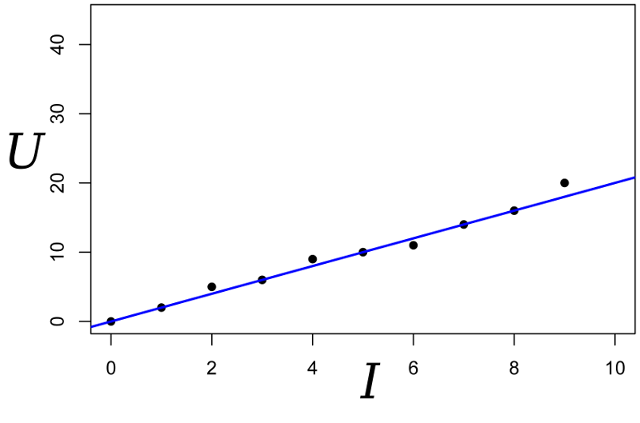
\includegraphics[width=.5\columnwidth]{URI}
\caption{Having $N$ meausrements $U_j$ for each reference current $I_j$, we are looking for the slope of the blue line that approximates the measurements through the Ohm's law.}
\label{fig:URI}
\end{figure}


Let us write the expression of the (logarithm of) likelihood of the parameters:
\begin{align*}
\log \mathcal{L}(R,\sigma) & = \log \left(\prod\limits_{j=1}^N  \frac{1}{\sqrt{2\pi}\sigma} \exp\left(-\frac{(U_j-R I_j)^2}{2\sigma^2}\right)\right) =\\
& = -N \left(\log\sqrt{2\pi} + \log\sigma\right) - \frac{1}{2\sigma^2} \sum\limits_{j=1}^N (U_j- R I_j)^2
\end{align*}

As usual, we equate the partial derivatives to zero:
\begin{align*}
\frac{\partial\log\mathcal{L}}{\partial R} &=  -\frac{1}{2\sigma^2}\sum\limits_{j=1}^N -2I_j (U_j- R I_j) = \\
&= \frac{1}{\sigma^2}\left(\sum\limits_{j=1}^N I_jU_j - R\sum\limits_{j=1}^N I_j^2\right) = 0
\end{align*}

Then the most plausible resistance $R$ can be found with the following formula:
$$
R = \frac{\sum\limits_{j=1}^N I_jU_j}{\sum\limits_{j=1}^N I_j^2}
$$

This result is somewhat less obvious than the simple average of all measurements in the previous example.
Note that if we take one hundred measurements with $\approx 1A$ reference current and one measurement with $\approx 1kA$ reference current,
then the first hundred measurements would barely affect the result. Let's remember this fact, we will need it later.

\subsection{Fourth example: back to the least squares}
You have probably already noticed that in the last two examples, maximizing the logarithm of the likelihood is equivalent to minimizing the sum of squared estimation errors.
Let us consider one more example.
Say we want to calibrate a spring scale with a help of reference weights.
Suppose we have $N$ reference weights of mass $x_j$; we weigh them with the scale and measure the length of the spring.
So, we have $N$ spring lengths $y_j$:
$$
\{x_j, y_j\}_{j=1}^{N}
$$

Hooke's law tells us that spring stretches linearly on the force applied;
this force includes the reference weight and the weight of the spring itself. 
Let us denote the spring stiffness as $a$, and the spring length streched under under its own weight as $b$. 
Then we can express the plausibility of our measurements (still under the Gaussian measurement noise hypothesis) in this way:
\begin{align*}
\log \mathcal{L}(a, b,\sigma) & = \log \left(\prod\limits_{j=1}^N  \frac{1}{\sqrt{2\pi}\sigma} \exp\left(-\frac{(y_j - a x_j - b)^2}{2\sigma^2}\right)\right) =\\
& = -N \left(\log\sqrt{2\pi} + \log\sigma\right) - \frac{1}{2\sigma^2} \sum\limits_{j=1}^N (y_j- a x_j - b)^2
\end{align*}

Maximizing the likelihood of $\mathcal L$ is equivalent to minimizing the sum of the squared estimation error, i.e., we are looking for the minimum of the function $S$ defined as follows:
$$
S(a, b) = \sum\limits_{j=1}^N (y_j- a x_j - b)^2
$$


\begin{figure}[htb!]
\centering
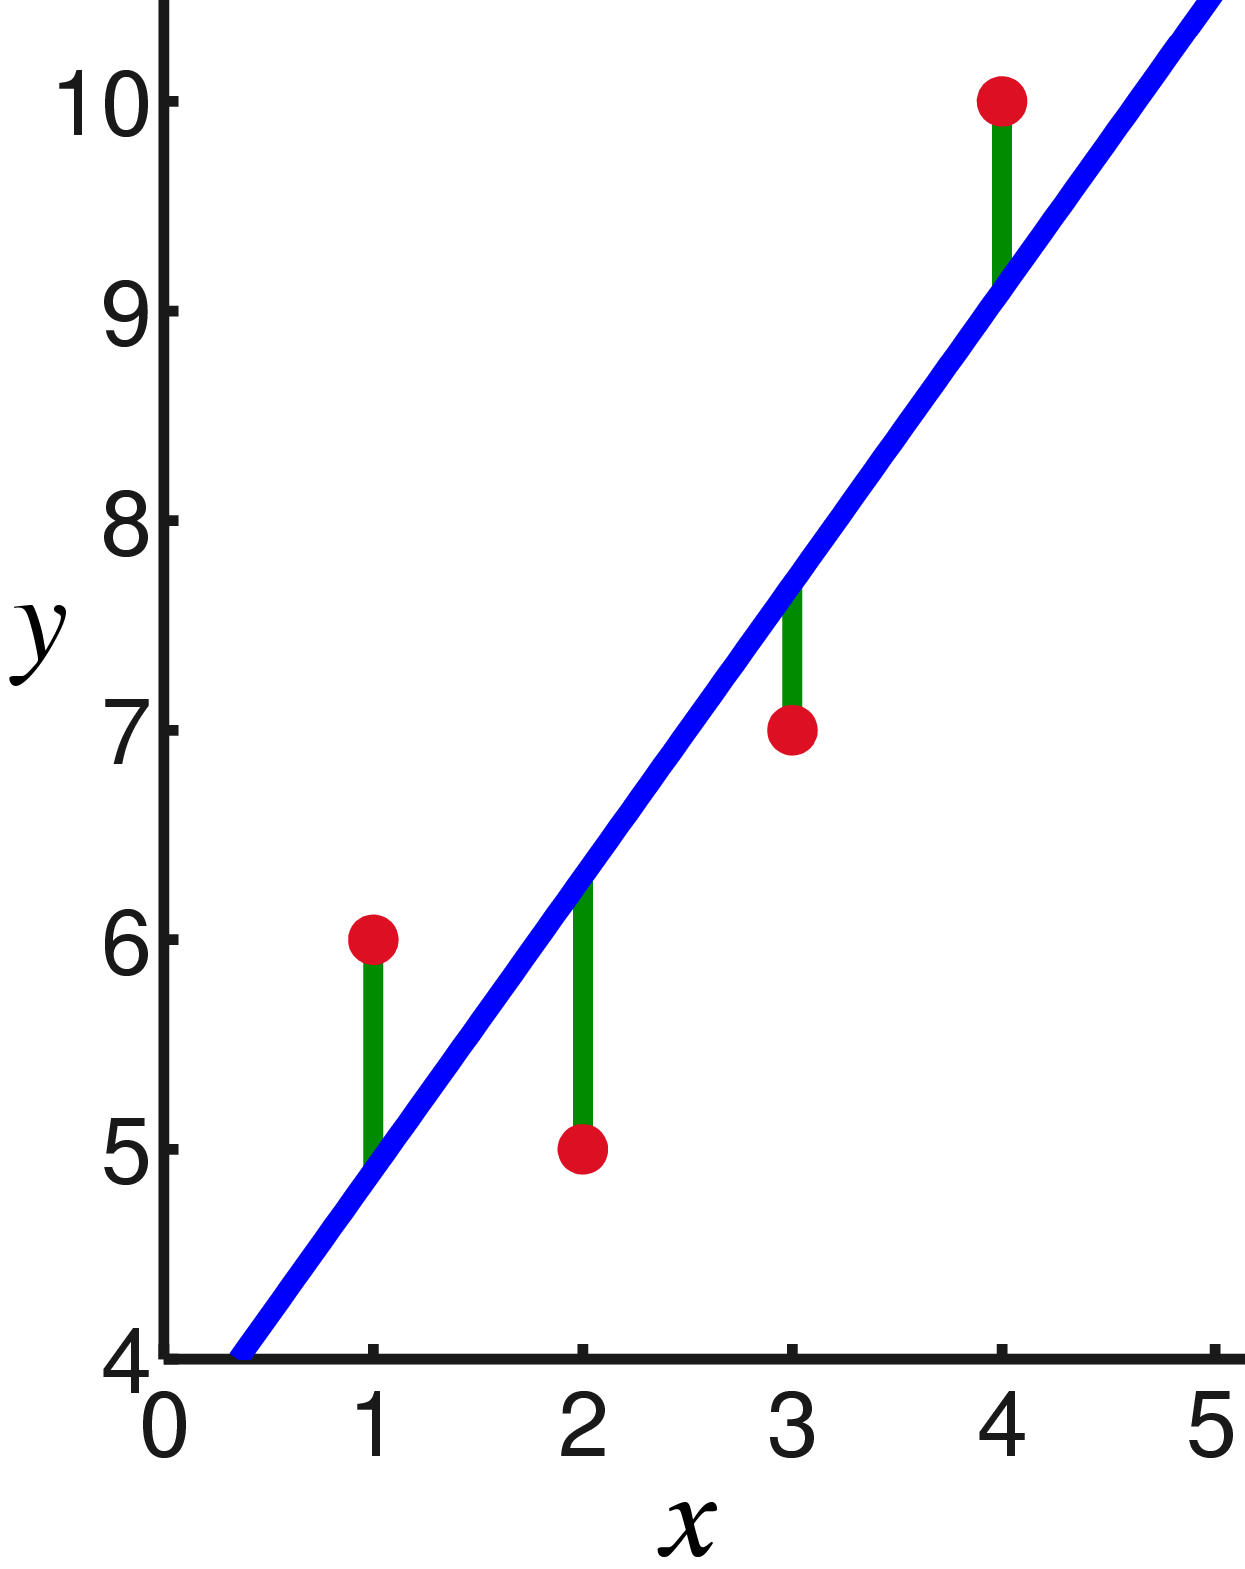
\includegraphics[width=.2\columnwidth]{c5aa80f6a2e9575abfa7b3dfdabf5c5a.png}
\caption{To calibrate the spring scale, we can solve the linear regression problem.}
\label{fig:regression}
\end{figure}

Figure~\ref{fig:regression} illustrates the formula: we are looking for such a straight line that minimizes the sum of squared lengths of green segments.
And then the derivation is quite straightforward:
\begin{align*}
\frac{\partial S}{\partial a} &= \sum\limits_{j=1}^N 2 x_j (a x_j + b - y_j) = 0 \\
\frac{\partial S}{\partial b} &= \sum\limits_{j=1}^N 2 (a x_j + b - y_j) = 0
\end{align*}

We obtain a system of two linear equations with two unknowns:
$$
\left \{ \begin{array}{r l}
a \sum\limits_{j=1}^N x_j^2 + b \sum\limits_{j=1}^N x_j  & = \sum\limits_{j=1}^N x_j y_j\\
a \sum\limits_{j=1}^N x_j   + b N                        & = \sum\limits_{j=1}^N y_j
\end{array} \right.
$$

Use your favorite method to obtain the following solution:
\begin{align*}
a &= \frac{N \sum\limits_{j=1}^N x_j y_j - \sum\limits_{j=1}^N x_j \sum\limits_{j=1}^N y_j}{N\sum\limits_{j=1}^N x_j^2 - \left(\sum\limits_{j=1}^N x_j\right)^2} \\
b &= \frac{1}{N}\left(  \sum\limits_{j=1}^N y_j - a  \sum\limits_{j=1}^N x_j \right)
\end{align*}

\subsection{Conclusion}
The least squares method is a particular case of maximizing likelihood in cases where the probability density is Gaussian.
If the density is not Gaussian, the least squares approach can produce an estimate different from the MLE (maximum likelihood estimation).
By the way, Gauss conjectured that the type of noise is of no importance, and the only thing that matters is the independence of trials.

As you have already noticed, the more we parameters we have, the more cumbersome the analytical solutions are.
Fortunately, we are not living in XVIII century anymore, we have computers!
Next we will try to build a geometric intuition on least squares, and see how can least squares problems be efficiently implemented.


\end{document}

